\chapter{Introducción y objetivo}
\label{ch:introduccion}

\section{Introducción}
La realidad aumentada es una tecnología que está en pleno auge, no paramos de ver noticias que nos muestran todo lo que esta permite, las diferentes utilizades que tiene y como va a mejorarnos la vida. No obstante esto no era así hace un año, como se puede observar en el grafico del "Hype Cycle" de Gartner sobre tecnologías emergentes en 2017, Figura \ref{figura-gartner}, la realidad aumentada se situaba en el tramo de desilusión, lo que significa que despues de estar en lo alto de la gráfica años anteriores, cuando se hablaba mucho de la tecnología y todo lo que ofrecía, en julio de 2017 se encontraba en lo mas bajo, apenas se hablaba de dicha tecnología, lo que significa que aun hay mucho por hacer, y queda mucho por trabajar sobre esta tecnología.\\

\begin{figure}[h]
  \centering
  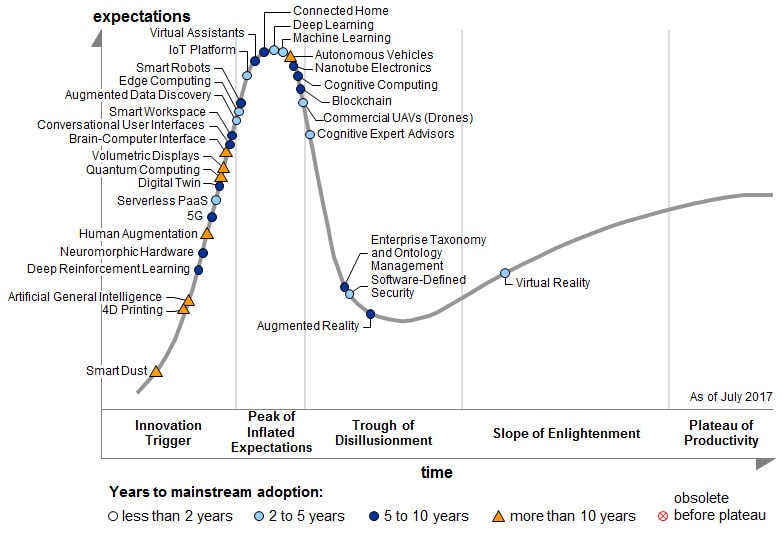
\includegraphics[scale=0.5]{gartner-hype-cycle}
  \caption{Imagen que muestra el "Hype cycle" de Gartner para tecnologías emergentes en 2017.\protect\footnotemark}
  \label{figura-gartner}
\end{figure}

\footnotetext{ \url{https://www.gartner.com/newsroom/id/3784363}, Gartner (July 2017)}

Sin embargo, desde que Apple y Google lanzaran sus respectivas librerías hace apenas un año, la realidad aumentada ha mejorado su situación notablemente, distanciándose de la realidad aumentada vista hasta el momento, estas nuevas librerias permiten, con los componentes de un dispositivo móvil de masas sea posible reconocer y entender el mundo que le rodea, así como su posición en el mundo. Esto supone una diferenciación en las tecnologías hasta entonces presentes, que o bien necesitaban de mucho hardware para ser capaces de conseguir esto, o en dispositivos móviles de masas, tenían capacidades reducidas.\\

Estas nuevas capacidades adquiridas

\newpage

\section{Motivación}

\section{Estructura del documento}
Este documento se divide en 4 capítulos, a continuación se detalla el contenido de cada uno de los capítulos del documento:
\begin{itemize}
  \item \textbf{Capítulo 1, Introducción y objetivo:} En este capítulo se hace una pequeña introducción al proyecto, explicando la motivación por la que surgió el proyecto, y también se exponen los objetivos que han sido establecidos para este proyecto.
  \item \textbf{Capítulo 2, Estado del arte:} En este capítulo se hará una exposición de cual es el estado actual de la realidad aumentada.
  \item \textbf{Capítulo 3, Proceso de desarrollo:} En este capítulo se detallará las metodologías de desarrollo utilizadas, la planificación del proyecto y el proceso de desarrollo del mismo.
  \item \textbf{Capítulo 4, Conclusiones finales y futuro:} En este capítulo se recoge el resultado del proyecto, las conclusiones obtenidas del desarrollo de éste y el trabajo futuro a realizar en el proyecto.
\end{itemize}

\section{Objetivo}
